\batchmode
\documentclass[12pt,leqno,]{article}
\RequirePackage{ifthen}


\usepackage{boxedminipage}


\bibliographystyle{plain_ep_doi_hr}


\usepackage{makeidx} 
\makeindex


\usepackage{html}


%
\renewcommand{\href}[2]{\url{#1}}  % putting #2 in looks like garbage

%
\providecommand{\bbm}{\vspace{5pt}

\noindent\begin{boxedminipage}{2.0\linewidth}}  

%
\providecommand{\maxlink}[1]{{http://maxima.sourceforge.net/docs/manual/en/}#1}%
\providecommand{\maxman}[2]{\htmladdnormallink{#1}{{http://maxima.sourceforge.net/docs/manual/en/}#2}}%
\providecommand{\umaxman}[2]{\htmladdnormallink{{\bf #1}}{{http://maxima.sourceforge.net/docs/manual/en/}#2}\maxcom\index{#1@{\bf #1}}}%
\providecommand{\imaxman}[2]{\htmladdnormallink{#1}{{http://maxima.sourceforge.net/docs/manual/en/}#2}\index{#1}} 

%
\providecommand{\hlink}[2]{\htmladdnormallink{#1}{#2}} 





\usepackage{graphicx}
\usepackage{hyperref}
\usepackage{verbatim}
\usepackage[cmbase]{flexisym}
\usepackage{bbold}


\usepackage{breqn}
\setkeys{breqn}{compact}

%
\providecommand{\ebm}{\end{boxedminipage}\vspace{5pt}

\noindent} 

\setlength{\fboxrule}{0.1pt}  

\setlength{\fboxsep}{10pt} 



\setlength{\textwidth}{180mm} 

\setlength{\oddsidemargin}{15mm} 

\addtolength{\oddsidemargin}{-1in} 

\setlength{\evensidemargin}{15mm} 

\addtolength{\evensidemargin}{-1in} 

%
\providecommand{\ifrac}[2]{\frac{#1}{#2}}%
\providecommand{\ifracd}[2]{\frac{#1}{#2}}%
\providecommand{\ifracn}[2]{\frac{#1}{#2}}%
\providecommand{\isubscript}[2]{{#1}_{#2}}%
\providecommand{\iexpt}[2]{{#1}^{#2}}%
\providecommand{\isqrt}[1]{\sqrt{#1}} 

%
\providecommand{\ket}[1]{{\lvert#1 \rangle}}%
\providecommand{\bra}[1]{{\langle#1 \rvert}}%
\providecommand{\bracket}[2]{{\langle#1|#2\rangle}}%
\providecommand{\func}[2]{{\bf #1}($#2$)}%
\providecommand{\marray}[2]{{\bf #1}[$#2$]}%
\providecommand{\fs}[1]{{\bf #1}} 

%
\providecommand{\ifs}[1]{ {\bf #1} \index{#1@{\bf #1}}}  % bold index entry plus bold in text

%
\providecommand{\ient}[1]{{#1}\index{#1}}  % index entry plus text%
\providecommand{\ibd}[1]{\index{#1@{\bf #1}}}  % bold index entry%
\providecommand{\iit}[1]{\index{#1@{\it #1}}}  % italic index entry%
\providecommand{\ipname}[1]{{\it #1}\index{#1@{\it #1}}}%
\providecommand{\pname}[1]{{\it #1}}  % software name%
\providecommand{\imarray}[2]{{\bf #1}[$#2$]\index{#1@{{\bf #1}[$#2$]}}}  % \marray with index entry%
\providecommand{\ifunc}[2]{{\bf #1}($#2$)\index{#1@{\bf #1}($#2$)}}  % \func with index entry%
\providecommand{\qinf}{ {\it qinf } }  % the name of this package%
\providecommand{\qinfp}{{\it qinf}}  % use at end of sentece for period

%
\providecommand{\farg}[1]{{\it #1}}  % an argument

%
\providecommand{\maximalink}{\htmladdnormallink{ {\it Maxima} }{http://maxima.sourceforge.net/}} 

%
\providecommand{\maxcom}{\textsuperscript{$\dagger$}} 




\usepackage[dvips]{color}


\pagecolor{white}

\usepackage[latin1]{inputenc}



\makeatletter

\makeatletter
\count@=\the\catcode`\_ \catcode`\_=8 
\newenvironment{tex2html_wrap}{}{}%
\catcode`\<=12\catcode`\_=\count@
\newcommand{\providedcommand}[1]{\expandafter\providecommand\csname #1\endcsname}%
\newcommand{\renewedcommand}[1]{\expandafter\providecommand\csname #1\endcsname{}%
  \expandafter\renewcommand\csname #1\endcsname}%
\newcommand{\newedenvironment}[1]{\newenvironment{#1}{}{}\renewenvironment{#1}}%
\let\newedcommand\renewedcommand
\let\renewedenvironment\newedenvironment
\makeatother
\let\mathon=$
\let\mathoff=$
\ifx\AtBeginDocument\undefined \newcommand{\AtBeginDocument}[1]{}\fi
\newbox\sizebox
\setlength{\hoffset}{0pt}\setlength{\voffset}{0pt}
\addtolength{\textheight}{\footskip}\setlength{\footskip}{0pt}
\addtolength{\textheight}{\topmargin}\setlength{\topmargin}{0pt}
\addtolength{\textheight}{\headheight}\setlength{\headheight}{0pt}
\addtolength{\textheight}{\headsep}\setlength{\headsep}{0pt}
\setlength{\textwidth}{349pt}
\newwrite\lthtmlwrite
\makeatletter
\let\realnormalsize=\normalsize
\global\topskip=2sp
\def\preveqno{}\let\real@float=\@float \let\realend@float=\end@float
\def\@float{\let\@savefreelist\@freelist\real@float}
\def\liih@math{\ifmmode$\else\bad@math\fi}
\def\end@float{\realend@float\global\let\@freelist\@savefreelist}
\let\real@dbflt=\@dbflt \let\end@dblfloat=\end@float
\let\@largefloatcheck=\relax
\let\if@boxedmulticols=\iftrue
\def\@dbflt{\let\@savefreelist\@freelist\real@dbflt}
\def\adjustnormalsize{\def\normalsize{\mathsurround=0pt \realnormalsize
 \parindent=0pt\abovedisplayskip=0pt\belowdisplayskip=0pt}%
 \def\phantompar{\csname par\endcsname}\normalsize}%
\def\lthtmltypeout#1{{\let\protect\string \immediate\write\lthtmlwrite{#1}}}%
\newcommand\lthtmlhboxmathA{\adjustnormalsize\setbox\sizebox=\hbox\bgroup\kern.05em }%
\newcommand\lthtmlhboxmathB{\adjustnormalsize\setbox\sizebox=\hbox to\hsize\bgroup\hfill }%
\newcommand\lthtmlvboxmathA{\adjustnormalsize\setbox\sizebox=\vbox\bgroup %
 \let\ifinner=\iffalse \let\)\liih@math }%
\newcommand\lthtmlboxmathZ{\@next\next\@currlist{}{\def\next{\voidb@x}}%
 \expandafter\box\next\egroup}%
\newcommand\lthtmlmathtype[1]{\gdef\lthtmlmathenv{#1}}%
\newcommand\lthtmllogmath{\dimen0\ht\sizebox \advance\dimen0\dp\sizebox
  \ifdim\dimen0>.95\vsize
   \lthtmltypeout{%
*** image for \lthtmlmathenv\space is too tall at \the\dimen0, reducing to .95 vsize ***}%
   \ht\sizebox.95\vsize \dp\sizebox\z@ \fi
  \lthtmltypeout{l2hSize %
:\lthtmlmathenv:\the\ht\sizebox::\the\dp\sizebox::\the\wd\sizebox.\preveqno}}%
\newcommand\lthtmlfigureA[1]{\let\@savefreelist\@freelist
       \lthtmlmathtype{#1}\lthtmlvboxmathA}%
\newcommand\lthtmlpictureA{\bgroup\catcode`\_=8 \lthtmlpictureB}%
\newcommand\lthtmlpictureB[1]{\lthtmlmathtype{#1}\egroup
       \let\@savefreelist\@freelist \lthtmlhboxmathB}%
\newcommand\lthtmlpictureZ[1]{\hfill\lthtmlfigureZ}%
\newcommand\lthtmlfigureZ{\lthtmlboxmathZ\lthtmllogmath\copy\sizebox
       \global\let\@freelist\@savefreelist}%
\newcommand\lthtmldisplayA{\bgroup\catcode`\_=8 \lthtmldisplayAi}%
\newcommand\lthtmldisplayAi[1]{\lthtmlmathtype{#1}\egroup\lthtmlvboxmathA}%
\newcommand\lthtmldisplayB[1]{\edef\preveqno{(\theequation)}%
  \lthtmldisplayA{#1}\let\@eqnnum\relax}%
\newcommand\lthtmldisplayZ{\lthtmlboxmathZ\lthtmllogmath\lthtmlsetmath}%
\newcommand\lthtmlinlinemathA{\bgroup\catcode`\_=8 \lthtmlinlinemathB}
\newcommand\lthtmlinlinemathB[1]{\lthtmlmathtype{#1}\egroup\lthtmlhboxmathA
  \vrule height1.5ex width0pt }%
\newcommand\lthtmlinlineA{\bgroup\catcode`\_=8 \lthtmlinlineB}%
\newcommand\lthtmlinlineB[1]{\lthtmlmathtype{#1}\egroup\lthtmlhboxmathA}%
\newcommand\lthtmlinlineZ{\egroup\expandafter\ifdim\dp\sizebox>0pt %
  \expandafter\centerinlinemath\fi\lthtmllogmath\lthtmlsetinline}
\newcommand\lthtmlinlinemathZ{\egroup\expandafter\ifdim\dp\sizebox>0pt %
  \expandafter\centerinlinemath\fi\lthtmllogmath\lthtmlsetmath}
\newcommand\lthtmlindisplaymathZ{\egroup %
  \centerinlinemath\lthtmllogmath\lthtmlsetmath}
\def\lthtmlsetinline{\hbox{\vrule width.1em \vtop{\vbox{%
  \kern.1em\copy\sizebox}\ifdim\dp\sizebox>0pt\kern.1em\else\kern.3pt\fi
  \ifdim\hsize>\wd\sizebox \hrule depth1pt\fi}}}
\def\lthtmlsetmath{\hbox{\vrule width.1em\kern-.05em\vtop{\vbox{%
  \kern.1em\kern0.9 pt\hbox{\hglue.17em\copy\sizebox\hglue0.9 pt}}\kern.3pt%
  \ifdim\dp\sizebox>0pt\kern.1em\fi \kern0.9 pt%
  \ifdim\hsize>\wd\sizebox \hrule depth1pt\fi}}}
\def\centerinlinemath{%
  \dimen1=\ifdim\ht\sizebox<\dp\sizebox \dp\sizebox\else\ht\sizebox\fi
  \advance\dimen1by.5pt \vrule width0pt height\dimen1 depth\dimen1 
 \dp\sizebox=\dimen1\ht\sizebox=\dimen1\relax}

\def\lthtmlcheckvsize{\ifdim\ht\sizebox<\vsize 
  \ifdim\wd\sizebox<\hsize\expandafter\hfill\fi \expandafter\vfill
  \else\expandafter\vss\fi}%
\providecommand{\selectlanguage}[1]{}%
\makeatletter \tracingstats = 1 


\begin{document}
\pagestyle{empty}\thispagestyle{empty}\lthtmltypeout{}%
\lthtmltypeout{latex2htmlLength hsize=\the\hsize}\lthtmltypeout{}%
\lthtmltypeout{latex2htmlLength vsize=\the\vsize}\lthtmltypeout{}%
\lthtmltypeout{latex2htmlLength hoffset=\the\hoffset}\lthtmltypeout{}%
\lthtmltypeout{latex2htmlLength voffset=\the\voffset}\lthtmltypeout{}%
\lthtmltypeout{latex2htmlLength topmargin=\the\topmargin}\lthtmltypeout{}%
\lthtmltypeout{latex2htmlLength topskip=\the\topskip}\lthtmltypeout{}%
\lthtmltypeout{latex2htmlLength headheight=\the\headheight}\lthtmltypeout{}%
\lthtmltypeout{latex2htmlLength headsep=\the\headsep}\lthtmltypeout{}%
\lthtmltypeout{latex2htmlLength parskip=\the\parskip}\lthtmltypeout{}%
\lthtmltypeout{latex2htmlLength oddsidemargin=\the\oddsidemargin}\lthtmltypeout{}%
\makeatletter
\if@twoside\lthtmltypeout{latex2htmlLength evensidemargin=\the\evensidemargin}%
\else\lthtmltypeout{latex2htmlLength evensidemargin=\the\oddsidemargin}\fi%
\lthtmltypeout{}%
\makeatother
\setcounter{page}{1}
\onecolumn

% !!! IMAGES START HERE !!!

\stepcounter{section}
\stepcounter{subsection}
\stepcounter{section}
{\newpage\clearpage
\lthtmlfigureA{boxedminipage4502}%
\begin{boxedminipage}{2.0\linewidth}
\begin{verbatim}

(%i1) 1 + 1;
\end{verbatim}

\begin{dmath}[number={\%o1}]
  2\end{dmath} 
\end{boxedminipage}%
\lthtmlfigureZ
\lthtmlcheckvsize\clearpage}

{\newpage\clearpage
\lthtmlfigureA{boxedminipage4513}%
\begin{boxedminipage}{2.0\linewidth}
\begin{verbatim}

(%i2) a : 2 * 2;
\end{verbatim}

\begin{dmath}[number={\%o2}]
 4\end{dmath}
\begin{verbatim}

(%i3) a;
\end{verbatim}

\begin{dmath}[number={\%o3}]
 4\end{dmath}
\begin{verbatim}

(%i4) b : expand( (x+y)^4 );
\end{verbatim}

\begin{dmath}[number={\%o4}]
 y^{4}+4\*x\*y^{3}+6\*x^{2}\*y^{2}+4\*x^{3}\*y+x^{4}\end{dmath}
\end{boxedminipage}%
\lthtmlfigureZ
\lthtmlcheckvsize\clearpage}

{\newpage\clearpage
\lthtmlfigureA{boxedminipage4520}%
\begin{boxedminipage}{2.0\linewidth}
\begin{verbatim}

(%i5) b : expand( (x+y)^50 )$
(%i6) length(b);
\end{verbatim}

\begin{dmath}[number={\%o6}]
 51\end{dmath}
\end{boxedminipage}%
\lthtmlfigureZ
\lthtmlcheckvsize\clearpage}

{\newpage\clearpage
\lthtmlfigureA{boxedminipage4528}%
\begin{boxedminipage}{2.0\linewidth}
\begin{verbatim}

(%i7)  1  + sqrt(2);
\end{verbatim}

\begin{dmath}[number={\%o7}]
 \sqrt{2}+1\end{dmath}

\begin{verbatim}

(%i8)  1  + sqrt(2), float;
\end{verbatim}

\begin{dmath}[number={\%o8}]
 2.4142135623730949\end{dmath}
\end{boxedminipage}%
\lthtmlfigureZ
\lthtmlcheckvsize\clearpage}

{\newpage\clearpage
\lthtmlfigureA{boxedminipage4537}%
\begin{boxedminipage}{2.0\linewidth}
\begin{verbatim}

(%i9) f(x) := 3 * cos(x);
\end{verbatim}

\begin{dmath}[number={\%o9}]
 f\left(x\right):=3\*\cos x\end{dmath}
\begin{verbatim}

(%i10) f(a);
\end{verbatim}

\begin{dmath}[number={\%o10}]
 3\*\cos 4\end{dmath}
\begin{verbatim}

(%i11) f(0);
\end{verbatim}

\begin{dmath}[number={\%o11}]
 3\end{dmath}
\end{boxedminipage}%
\lthtmlfigureZ
\lthtmlcheckvsize\clearpage}

{\newpage\clearpage
\lthtmlfigureA{boxedminipage4545}%
\begin{boxedminipage}{2.0\linewidth}
\begin{verbatim}

(%i12) expand ( (1 + 2 * %i)^2 );
\end{verbatim}

\begin{dmath}[number={\%o12}]
 4\*i-3\end{dmath}
\end{boxedminipage}%
\lthtmlfigureZ
\lthtmlcheckvsize\clearpage}

{\newpage\clearpage
\lthtmlfigureA{boxedminipage4550}%
\begin{boxedminipage}{2.0\linewidth}
\begin{verbatim}

(%i13) cos(%pi/2);
\end{verbatim}

\begin{dmath}[number={\%o13}]
 0\end{dmath}
\begin{verbatim}

(%i14) %e^(%i * %pi/2);
\end{verbatim}

\begin{dmath}[number={\%o14}]
 i\end{dmath}
\end{boxedminipage}%
\lthtmlfigureZ
\lthtmlcheckvsize\clearpage}

\stepcounter{section}
\stepcounter{section}
\stepcounter{subsection}
{\newpage\clearpage
\lthtmlfigureA{boxedminipage4586}%
\begin{boxedminipage}{2.0\linewidth}
\begin{verbatim}

(%i3) ketz(1)
\end{verbatim}

\begin{dmath}[number={\%o3}]
 \pmatrix{0\cr 1\cr }\end{dmath}
\end{boxedminipage}%
\lthtmlfigureZ
\lthtmlcheckvsize\clearpage}

{\newpage\clearpage
\lthtmlfigureA{boxedminipage4591}%
\begin{boxedminipage}{2.0\linewidth}
\begin{verbatim}

(%i4) braz(1)
\end{verbatim}

\begin{dmath}[number={\%o4}]
 \pmatrix{0&\linebreak[0]1\cr }\end{dmath}
\end{boxedminipage}%
\lthtmlfigureZ
\lthtmlcheckvsize\clearpage}

{\newpage\clearpage
\lthtmlfigureA{boxedminipage4596}%
\begin{boxedminipage}{2.0\linewidth}
\begin{verbatim}

(%i5) braz(0)
\end{verbatim}

\begin{dmath}[number={\%o5}]
 \pmatrix{1&\linebreak[0]0\cr }\end{dmath}
\end{boxedminipage}%
\lthtmlfigureZ
\lthtmlcheckvsize\clearpage}

{\newpage\clearpage
\lthtmlfigureA{boxedminipage4605}%
\begin{boxedminipage}{2.0\linewidth}
\begin{verbatim}

(%i6) braz(0,0)
\end{verbatim}

\begin{dmath}[number={\%o6}]
 \pmatrix{1&\linebreak[0]0&\linebreak[0]0&\linebreak[0]0\cr }\end{dmath}
\begin{verbatim}

(%i7) braz(1,1)
\end{verbatim}

\begin{dmath}[number={\%o7}]
 \pmatrix{0&\linebreak[0]0&\linebreak[0]0&\linebreak[0]1\cr }\end{dmath}
\begin{verbatim}

(%i8) alpha[1]*braz(1,1)+alpha[0]*braz(0,0)
\end{verbatim}

\begin{dmath}[number={\%o8}]
 \pmatrix{\alpha_{0}&\linebreak[0]0&\linebreak[0]0&\linebreak[0]\alpha_{1}\cr }\end{dmath}
\end{boxedminipage}%
\lthtmlfigureZ
\lthtmlcheckvsize\clearpage}

{\newpage\clearpage
\lthtmlfigureA{boxedminipage4622}%
\begin{boxedminipage}{2.0\linewidth}
\begin{verbatim}

(%i9) brax(1)
\end{verbatim}

\begin{dmath}[number={\%o9}]
 \pmatrix{\frac{1}{\sqrt{2}}&\linebreak[0]-\frac{1}{\sqrt{2}}\cr }\end{dmath}
\begin{verbatim}

(%i10) bray(1,0,1)
\end{verbatim}

\begin{dmath}[number={\%o10}]
 \pmatrix{\frac{1}{2\*\sqrt{2}}&\linebreak[0]\frac{i}{2\*\sqrt{2}}&\linebreak[0]-\frac{i}{2\*\sqrt{2}}&\linebreak[0]\frac{1}{2\*\sqrt{2}}&\linebreak[0]\frac{i}{2\*\sqrt{2}}&\linebreak[0]-\frac{1}{2\*\sqrt{2}}&\linebreak[0]\frac{1}{2\*\sqrt{2}}&\linebreak[0]\frac{i}{2\*\sqrt{2}}\cr }\end{dmath}
\end{boxedminipage}%
\lthtmlfigureZ
\lthtmlcheckvsize\clearpage}

\stepcounter{subsection}
\stepcounter{subsection}
{\newpage\clearpage
\lthtmlfigureA{boxedminipage4694}%
\begin{boxedminipage}{2.0\linewidth}
\begin{verbatim}

(%i19) ketx(1) . brax(1);
\end{verbatim}

\begin{dmath}[number={\%o19}]
 \pmatrix{\frac{1}{2}&\linebreak[0]-\frac{1}{2}\cr -\frac{1}{2}&\linebreak[0]\frac{1}{2}\cr }\end{dmath}
\end{boxedminipage}%
\lthtmlfigureZ
\lthtmlcheckvsize\clearpage}

{\newpage\clearpage
\lthtmlfigureA{boxedminipage4699}%
\begin{boxedminipage}{2.0\linewidth}
\begin{verbatim}

(%i20) brax(1) . ketx(1);
\end{verbatim}

\begin{dmath}[number={\%o20}]
 1\end{dmath}
\end{boxedminipage}%
\lthtmlfigureZ
\lthtmlcheckvsize\clearpage}

{\newpage\clearpage
\lthtmlfigureA{boxedminipage4708}%
\begin{boxedminipage}{2.0\linewidth}
\begin{verbatim}

(%i21) is ( ketz(0,0,0) . braz(0,0,0) =  ketz(0,0,0) . ctranspose(ketz(0,0,0)) );
\end{verbatim}

\begin{dmath}[number={\%o21}]
 \mathbf{true}\end{dmath}
\begin{verbatim}

(%i22) is ( ketz(1,0,1) . braz(1,0,1) =  proj(ketz(1,0,1)) );
\end{verbatim}

\begin{dmath}[number={\%o22}]
 \mathbf{true}\end{dmath}
\end{boxedminipage}%
\lthtmlfigureZ
\lthtmlcheckvsize\clearpage}

{\newpage\clearpage
\lthtmlfigureA{boxedminipage4730}%
\begin{boxedminipage}{2.0\linewidth}
\begin{verbatim}

(%i17) is ( tovect( proj(schmidt_ket(alpha))) = schmidt_ket(alpha));
\end{verbatim}

\begin{dmath}[number={\%o17}]
 \mathbf{true}\end{dmath}
\end{boxedminipage}%
\lthtmlfigureZ
\lthtmlcheckvsize\clearpage}

\stepcounter{subsection}
{\newpage\clearpage
\lthtmlfigureA{boxedminipage4756}%
\begin{boxedminipage}{2.0\linewidth}
\begin{verbatim}

(%i12) is (ketz(0,1) = ketz(0) otimes ketz(1))
\end{verbatim}

\begin{dmath}[number={\%o12}]
 \mathbf{true}\end{dmath}
\begin{verbatim}

(%i13) is (ketz(0,1) = tensor_product(ketz(0),ketz(1)))
\end{verbatim}

\begin{dmath}[number={\%o13}]
 \mathbf{true}\end{dmath}
\begin{verbatim}

(%i14) is (ketx(0,1,0) otimes kety(1,0,1)
            = tensor_product(ketx(0),ketx(1),ketx(0),kety(1),kety(0),kety(1)))\end{verbatim}

\begin{dmath}[number={\%o14}]
 \mathbf{true}\end{dmath}
\end{boxedminipage}%
\lthtmlfigureZ
\lthtmlcheckvsize\clearpage}

\stepcounter{subsection}
\stepcounter{subsection}
{\newpage\clearpage
\lthtmlfigureA{boxedminipage4799}%
\begin{boxedminipage}{2.0\linewidth}
\begin{verbatim}

(%i2) f[x,y] := belln[x] . belln[y];
\end{verbatim}

\begin{dmath}[number={\%o2}]
 f_{x,\linebreak[0]y}:=\mathrm{belln}_{x}\cdot \mathrm{belln}_{y}\end{dmath}
\end{boxedminipage}%
\lthtmlfigureZ
\lthtmlcheckvsize\clearpage}

{\newpage\clearpage
\lthtmlfigureA{boxedminipage4813}%
\begin{boxedminipage}{2.0\linewidth}
\begin{verbatim}

(%i3) genmatrix( f , 3,3,0,0);
\end{verbatim}

\begin{dmath}[number={\%o3}]
  \pmatrix{1&\linebreak[0]0&\linebreak[0]0&\linebreak[0]0\cr
    0&\linebreak[0]1&\linebreak[0]0&\linebreak[0]0\cr
    0&\linebreak[0]0&\linebreak[0]1&\linebreak[0]0\cr
    0&\linebreak[0]0&\linebreak[0]0&\linebreak[0]1\cr
  }\end{dmath}
\end{boxedminipage}%
\lthtmlfigureZ
\lthtmlcheckvsize\clearpage}

{\newpage\clearpage
\lthtmlfigureA{boxedminipage4844}%
\begin{boxedminipage}{2.0\linewidth}
\begin{verbatim}

(%i5) identitymatrixp(%);
\end{verbatim}

\begin{dmath}[number={\%o5}]
 \mathbf{true}\end{dmath}
\end{boxedminipage}%
\lthtmlfigureZ
\lthtmlcheckvsize\clearpage}

{\newpage\clearpage
\lthtmlfigureA{boxedminipage4849}%
\begin{boxedminipage}{2.0\linewidth}
\begin{verbatim}

(%i6) identitymatrixp(genmatrix( lambda( [x,y], belln[x] . belln[y]) , 3,3,0,0));
\end{verbatim}

\begin{dmath}[number={\%o6}]
 \mathbf{true}\end{dmath}
\end{boxedminipage}%
\lthtmlfigureZ
\lthtmlcheckvsize\clearpage}

{\newpage\clearpage
\lthtmlfigureA{boxedminipage4870}%
\begin{boxedminipage}{2.0\linewidth}
\begin{verbatim}

(%i2) identitymatrixp(apply("+",map(lambda([i],proj(belln[i])),[0,1,2,3])));
\end{verbatim}

\begin{dmath}[number={\%o2}]
 \mathbf{true}\end{dmath}
\end{boxedminipage}%
\lthtmlfigureZ
\lthtmlcheckvsize\clearpage}

\stepcounter{subsection}
\stepcounter{subsection}
{\newpage\clearpage
\lthtmlfigureA{boxedminipage4895}%
\begin{boxedminipage}{2.0\linewidth}
\begin{verbatim}

(%i2) wxplot2d(entropy(werner(a,1,0)), [a,0,1]);
\end{verbatim}

\begin{dmath}[number={\%o2}]
 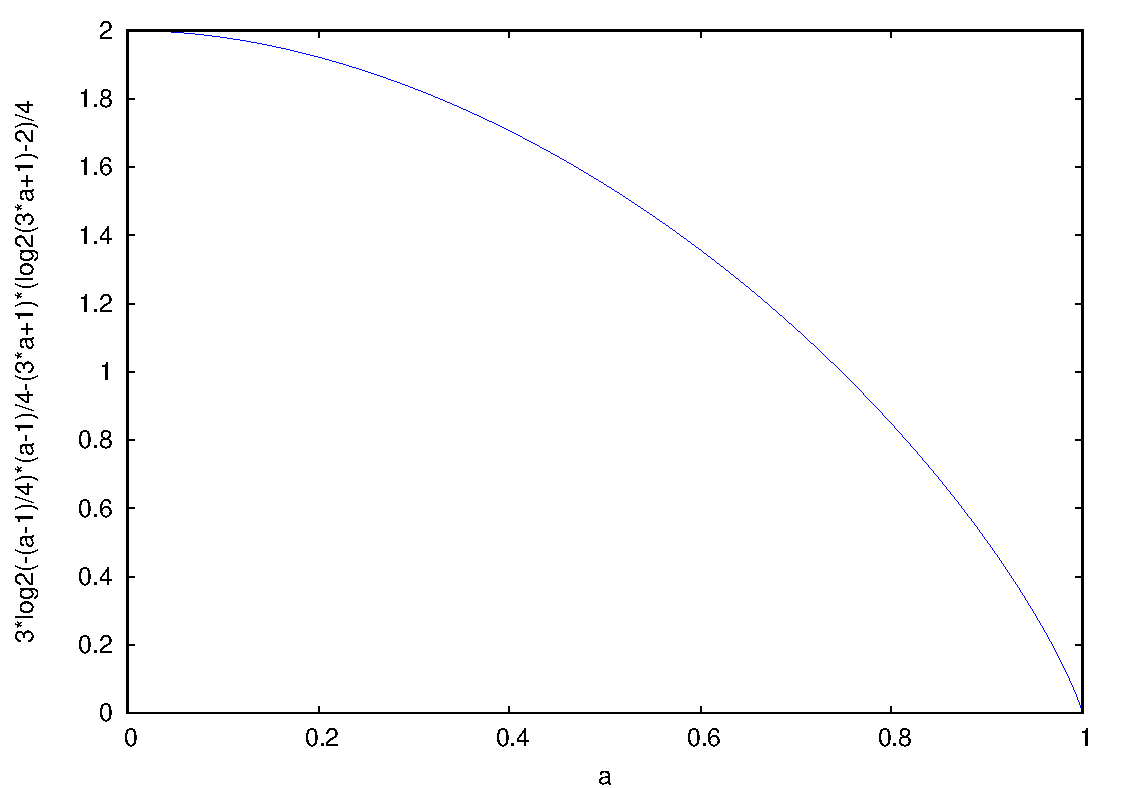
\includegraphics[width=.5\linewidth]{figs/werner_entropy}
\end{dmath}
\end{boxedminipage}%
\lthtmlfigureZ
\lthtmlcheckvsize\clearpage}

\stepcounter{section}
\stepcounter{subsection}
\stepcounter{subsubsection}
{\newpage\clearpage
\lthtmlfigureA{boxedminipage4904}%
\begin{boxedminipage}{2.0\linewidth}
\begin{verbatim}

(%i12) [ pauli[0], pauli[1], pauli[2], pauli[3] ];
\end{verbatim}

\begin{dmath}[number={\%o12}]
 \left[ \pmatrix{1&\linebreak[0]0\cr 0&\linebreak[0]1\cr },\linebreak[0]\pmatrix{0&\linebreak[0]1\cr 1&\linebreak[0]0\cr },\linebreak[0]\pmatrix{0&\linebreak[0]-i\cr i&\linebreak[0]0\cr },\linebreak[0]\pmatrix{1&\linebreak[0]0\cr 0&\linebreak[0]-1\cr } \right] \end{dmath}
\end{boxedminipage}%
\lthtmlfigureZ
\lthtmlcheckvsize\clearpage}

{\newpage\clearpage
\lthtmlfigureA{boxedminipage4910}%
\begin{boxedminipage}{2.0\linewidth}
\begin{verbatim}

(%i8) is (  pauli[1] . ket_n(1,1) = -1 * ket_n(1,1) );
\end{verbatim}

\begin{dmath}[number={\%o8}]
 \mathbf{true}\end{dmath}
\end{boxedminipage}%
\lthtmlfigureZ
\lthtmlcheckvsize\clearpage}

{\newpage\clearpage
\lthtmlfigureA{boxedminipage4915}%
\begin{boxedminipage}{2.0\linewidth}
\begin{verbatim}

(%i9) mapapply( lambda([i,j], is (pauli[i] . ket_n(i,j) = (-1)^j * ket_n(i,j))),
         [[1,0],[1,1],[2,0],[2,1],[3,0],[3,1]  ]);\end{verbatim}

\begin{dmath}[number={\%o9}]
 \left[ \mathbf{true},\linebreak[0]\mathbf{true},\linebreak[0]\mathbf{true},\linebreak[0]\mathbf{true},\linebreak[0]\mathbf{true},\linebreak[0]\mathbf{true} \right] \end{dmath}
\end{boxedminipage}%
\lthtmlfigureZ
\lthtmlcheckvsize\clearpage}

{\newpage\clearpage
\lthtmlfigureA{boxedminipage4938}%
\begin{boxedminipage}{2.0\linewidth}
\begin{verbatim}

(%i4) identitymatrixp( mat_unblocker (genmatrix(lambda([i,j],  
         anticommutator(pauli[i],pauli[j])/2 ), 3,3,1,1)));\end{verbatim}

\begin{dmath}[number={\%o4}]
  \mathbf{true}\end{dmath} \end{boxedminipage}%
\lthtmlfigureZ
\lthtmlcheckvsize\clearpage}

{\newpage\clearpage
\lthtmlfigureA{boxedminipage4977}%
\begin{boxedminipage}{2.0\linewidth}
\begin{verbatim}

(%i5) load("itensor");
\end{verbatim}

\begin{dmath}[number={\%o5}]
 \verb|/usr/share/maxima/5.15.0/share/tensor/itensor.lisp|\end{dmath}
\begin{verbatim}

(%i6) mapapply(lambda([i,j,k],zeromatrixp(commutator(pauli[i],pauli[j]) 
     - 2*%i*levi_civita([i,j,k])*pauli[k])), listify(permutations([1,2,3])));
\end{verbatim}

\begin{dmath}[number={\%o6}]
 \left[ \mathbf{true},\linebreak[0]\mathbf{true},\linebreak[0]\mathbf{true},\linebreak[0]\mathbf{true},\linebreak[0]\mathbf{true},\linebreak[0]\mathbf{true} \right] \end{dmath}
\end{boxedminipage}%
\lthtmlfigureZ
\lthtmlcheckvsize\clearpage}

\stepcounter{subsubsection}
\stepcounter{subsubsection}
\stepcounter{subsubsection}
\stepcounter{subsubsection}
\stepcounter{subsubsection}
{\newpage\clearpage
\lthtmlfigureA{boxedminipage5007}%
\begin{boxedminipage}{2.0\linewidth}
\begin{verbatim}

(%i2) m1 : matrix([a1,b1],[c1,d1]);
\end{verbatim}

\begin{dmath}[number={\%o2}]
 \pmatrix{\mathrm{a1}&\linebreak[0]\mathrm{b1}\cr \mathrm{c1}&\linebreak[0]\mathrm{d1}\cr }\end{dmath}
\begin{verbatim}

(%i3) m2 : matrix([a2,b2],[c2,d2]) $
(%i4) m3 : matrix([a3,b3],[c3,d3]) $
\end{verbatim}

\end{boxedminipage}%
\lthtmlfigureZ
\lthtmlcheckvsize\clearpage}

{\newpage\clearpage
\lthtmlfigureA{boxedminipage5012}%
\begin{boxedminipage}{2.0\linewidth}
\begin{verbatim}

(%i5) mp : m1 otimes m2 otimes  m3 ;
\end{verbatim}

\begin{dmath}[number={\%o5}]
 \pmatrix{\mathrm{a1}\*\mathrm{a2}\*\mathrm{a3}&\linebreak[0]\mathrm{a1}\*\mathrm{a2}\*\mathrm{b3}&\linebreak[0]\mathrm{a1}\*\mathrm{a3}\*\mathrm{b2}&\linebreak[0]\mathrm{a1}\*\mathrm{b2}\*\mathrm{b3}&\linebreak[0]\mathrm{a2}\*\mathrm{a3}\*\mathrm{b1}&\linebreak[0]\mathrm{a2}\*\mathrm{b1}\*\mathrm{b3}&\linebreak[0]\mathrm{a3}\*\mathrm{b1}\*\mathrm{b2}&\linebreak[0]\mathrm{b1}\*\mathrm{b2}\*\mathrm{b3}\cr \mathrm{a1}\*\mathrm{a2}\*\mathrm{c3}&\linebreak[0]\mathrm{a1}\*\mathrm{a2}\*\mathrm{d3}&\linebreak[0]\mathrm{a1}\*\mathrm{b2}\*\mathrm{c3}&\linebreak[0]\mathrm{a1}\*\mathrm{b2}\*\mathrm{d3}&\linebreak[0]\mathrm{a2}\*\mathrm{b1}\*\mathrm{c3}&\linebreak[0]\mathrm{a2}\*\mathrm{b1}\*\mathrm{d3}&\linebreak[0]\mathrm{b1}\*\mathrm{b2}\*\mathrm{c3}&\linebreak[0]\mathrm{b1}\*\mathrm{b2}\*\mathrm{d3}\cr \mathrm{a1}\*\mathrm{a3}\*\mathrm{c2}&\linebreak[0]\mathrm{a1}\*\mathrm{b3}\*\mathrm{c2}&\linebreak[0]\mathrm{a1}\*\mathrm{a3}\*\mathrm{d2}&\linebreak[0]\mathrm{a1}\*\mathrm{b3}\*\mathrm{d2}&\linebreak[0]\mathrm{a3}\*\mathrm{b1}\*\mathrm{c2}&\linebreak[0]\mathrm{b1}\*\mathrm{b3}\*\mathrm{c2}&\linebreak[0]\mathrm{a3}\*\mathrm{b1}\*\mathrm{d2}&\linebreak[0]\mathrm{b1}\*\mathrm{b3}\*\mathrm{d2}\cr \mathrm{a1}\*\mathrm{c2}\*\mathrm{c3}&\linebreak[0]\mathrm{a1}\*\mathrm{c2}\*\mathrm{d3}&\linebreak[0]\mathrm{a1}\*\mathrm{c3}\*\mathrm{d2}&\linebreak[0]\mathrm{a1}\*\mathrm{d2}\*\mathrm{d3}&\linebreak[0]\mathrm{b1}\*\mathrm{c2}\*\mathrm{c3}&\linebreak[0]\mathrm{b1}\*\mathrm{c2}\*\mathrm{d3}&\linebreak[0]\mathrm{b1}\*\mathrm{c3}\*\mathrm{d2}&\linebreak[0]\mathrm{b1}\*\mathrm{d2}\*\mathrm{d3}\cr \mathrm{a2}\*\mathrm{a3}\*\mathrm{c1}&\linebreak[0]\mathrm{a2}\*\mathrm{b3}\*\mathrm{c1}&\linebreak[0]\mathrm{a3}\*\mathrm{b2}\*\mathrm{c1}&\linebreak[0]\mathrm{b2}\*\mathrm{b3}\*\mathrm{c1}&\linebreak[0]\mathrm{a2}\*\mathrm{a3}\*\mathrm{d1}&\linebreak[0]\mathrm{a2}\*\mathrm{b3}\*\mathrm{d1}&\linebreak[0]\mathrm{a3}\*\mathrm{b2}\*\mathrm{d1}&\linebreak[0]\mathrm{b2}\*\mathrm{b3}\*\mathrm{d1}\cr \mathrm{a2}\*\mathrm{c1}\*\mathrm{c3}&\linebreak[0]\mathrm{a2}\*\mathrm{c1}\*\mathrm{d3}&\linebreak[0]\mathrm{b2}\*\mathrm{c1}\*\mathrm{c3}&\linebreak[0]\mathrm{b2}\*\mathrm{c1}\*\mathrm{d3}&\linebreak[0]\mathrm{a2}\*\mathrm{c3}\*\mathrm{d1}&\linebreak[0]\mathrm{a2}\*\mathrm{d1}\*\mathrm{d3}&\linebreak[0]\mathrm{b2}\*\mathrm{c3}\*\mathrm{d1}&\linebreak[0]\mathrm{b2}\*\mathrm{d1}\*\mathrm{d3}\cr \mathrm{a3}\*\mathrm{c1}\*\mathrm{c2}&\linebreak[0]\mathrm{b3}\*\mathrm{c1}\*\mathrm{c2}&\linebreak[0]\mathrm{a3}\*\mathrm{c1}\*\mathrm{d2}&\linebreak[0]\mathrm{b3}\*\mathrm{c1}\*\mathrm{d2}&\linebreak[0]\mathrm{a3}\*\mathrm{c2}\*\mathrm{d1}&\linebreak[0]\mathrm{b3}\*\mathrm{c2}\*\mathrm{d1}&\linebreak[0]\mathrm{a3}\*\mathrm{d1}\*\mathrm{d2}&\linebreak[0]\mathrm{b3}\*\mathrm{d1}\*\mathrm{d2}\cr \mathrm{c1}\*\mathrm{c2}\*\mathrm{c3}&\linebreak[0]\mathrm{c1}\*\mathrm{c2}\*\mathrm{d3}&\linebreak[0]\mathrm{c1}\*\mathrm{c3}\*\mathrm{d2}&\linebreak[0]\mathrm{c1}\*\mathrm{d2}\*\mathrm{d3}&\linebreak[0]\mathrm{c2}\*\mathrm{c3}\*\mathrm{d1}&\linebreak[0]\mathrm{c2}\*\mathrm{d1}\*\mathrm{d3}&\linebreak[0]\mathrm{c3}\*\mathrm{d1}\*\mathrm{d2}&\linebreak[0]\mathrm{d1}\*\mathrm{d2}\*\mathrm{d3}\cr }\end{dmath}
\end{boxedminipage}%
\lthtmlfigureZ
\lthtmlcheckvsize\clearpage}

{\newpage\clearpage
\lthtmlfigureA{boxedminipage5017}%
\begin{boxedminipage}{2.0\linewidth}
\begin{verbatim}

(%i6) pe : pauliexp(mp) $
\end{verbatim}

\end{boxedminipage}%
\lthtmlfigureZ
\lthtmlcheckvsize\clearpage}

{\newpage\clearpage
\lthtmlfigureA{boxedminipage5022}%
\begin{boxedminipage}{2.0\linewidth}
\begin{verbatim}

(%i7) length(pe);
\end{verbatim}

\begin{dmath}[number={\%o7}]
 64\end{dmath}
\begin{verbatim}

(%i8) part(pe,10);
\end{verbatim}

\begin{dmath}[number={\%o8}]
 \frac{-i\*\mathrm{c1}\*\mathrm{c2}\*\mathrm{d3}-i\*\mathrm{b1}\*\mathrm{c2}\*\mathrm{d3}+i\*\mathrm{b2}\*\mathrm{c1}\*\mathrm{d3}+i\*\mathrm{b1}\*\mathrm{b2}\*\mathrm{d3}-i\*\mathrm{a3}\*\mathrm{c1}\*\mathrm{c2}-i\*\mathrm{a3}\*\mathrm{b1}\*\mathrm{c2}+i\*\mathrm{a3}\*\mathrm{b2}\*\mathrm{c1}+i\*\mathrm{a3}\*\mathrm{b1}\*\mathrm{b2}}{8}\end{dmath}
\end{boxedminipage}%
\lthtmlfigureZ
\lthtmlcheckvsize\clearpage}

{\newpage\clearpage
\lthtmlfigureA{boxedminipage5053}%
\begin{boxedminipage}{2.0\linewidth}
\begin{verbatim}

(%i9) is ( ratsimp( invpauliexp( pauliexp(mp) )) = mp);
\end{verbatim}

\begin{dmath}[number={\%o9}]
 \mathbf{true}\end{dmath}
\end{boxedminipage}%
\lthtmlfigureZ
\lthtmlcheckvsize\clearpage}

{\newpage\clearpage
\lthtmlfigureA{boxedminipage5058}%
\begin{boxedminipage}{2.0\linewidth}
\begin{verbatim}

(%i10) correlation_tensor(pe,1,2,3);
\end{verbatim}

\begin{dmath}[number={\%o10}]
 \frac{i\*\mathrm{c1}\*\mathrm{c2}\*\mathrm{d3}+i\*\mathrm{b1}\*\mathrm{c2}\*\mathrm{d3}-i\*\mathrm{b2}\*\mathrm{c1}\*\mathrm{d3}-i\*\mathrm{b1}\*\mathrm{b2}\*\mathrm{d3}-i\*\mathrm{a3}\*\mathrm{c1}\*\mathrm{c2}-i\*\mathrm{a3}\*\mathrm{b1}\*\mathrm{c2}+i\*\mathrm{a3}\*\mathrm{b2}\*\mathrm{c1}+i\*\mathrm{a3}\*\mathrm{b1}\*\mathrm{b2}}{8}\end{dmath}
\end{boxedminipage}%
\lthtmlfigureZ
\lthtmlcheckvsize\clearpage}

\stepcounter{subsection}
{\newpage\clearpage
\lthtmlfigureA{boxedminipage5100}%
\begin{boxedminipage}{2.0\linewidth}
\begin{verbatim}

(%i2) spinor_rotation(phi,theta,gamma);
\end{verbatim}

\begin{dmath}[number={\%o2}]
 \pmatrix{\cos \left(\frac{\gamma}{2}\right)-i\*\cos \vartheta\*\sin \left(\frac{\gamma}{2}\right)&\linebreak[0]-i\*{e}^{- i\*\varphi }\*\sin \vartheta\*\sin \left(\frac{\gamma}{2}\right)\cr -i\*{e}^{i\*\varphi}\*\sin \vartheta\*\sin \left(\frac{\gamma}{2}\right)&\linebreak[0]i\*\cos \vartheta\*\sin \left(\frac{\gamma}{2}\right)+\cos \left(\frac{\gamma}{2}\right)\cr }\end{dmath}
\begin{verbatim}

(%i3) spinor_rotation_trig(phi,theta,gamma);
\end{verbatim}

\begin{dmath}[number={\%o3}]
 \pmatrix{\cos \left(\frac{\gamma}{2}\right)-i\*\cos \vartheta\*\sin \left(\frac{\gamma}{2}\right)&\linebreak[0]\left(-\sin \varphi\*\sin \vartheta-i\*\cos \varphi\*\sin \vartheta\right)\*\sin \left(\frac{\gamma}{2}\right)\cr \left(\sin \varphi\*\sin \vartheta-i\*\cos \varphi\*\sin \vartheta\right)\*\sin \left(\frac{\gamma}{2}\right)&\linebreak[0]i\*\cos \vartheta\*\sin \left(\frac{\gamma}{2}\right)+\cos \left(\frac{\gamma}{2}\right)\cr }\end{dmath}.
\end{boxedminipage}%
\lthtmlfigureZ
\lthtmlcheckvsize\clearpage}

\stepcounter{subsection}
\stepcounter{subsection}
\stepcounter{subsubsection}
{\newpage\clearpage
\lthtmlfigureA{boxedminipage5121}%
\begin{boxedminipage}{2.0\linewidth}
\begin{verbatim}

(%i2) hadamard;
\end{verbatim}

\begin{dmath}[number={\%o2}]
 \pmatrix{\frac{1}{\sqrt{2}}&\linebreak[0]\frac{1}{\sqrt{2}}\cr \frac{1}{\sqrt{2}}&\linebreak[0]-\frac{1}{\sqrt{2}}\cr }\end{dmath}
\end{boxedminipage}%
\lthtmlfigureZ
\lthtmlcheckvsize\clearpage}

\stepcounter{subsubsection}
\stepcounter{subsubsection}
\stepcounter{subsubsection}
\stepcounter{subsubsection}
\stepcounter{subsubsection}
\stepcounter{section}
\stepcounter{subsection}
{\newpage\clearpage
\lthtmlfigureA{boxedminipage5223}%
\begin{boxedminipage}{2.0\linewidth}
\begin{verbatim}

(%i1) m1 : matrix([a1,b1,c1],[d1,e1,f1],[g1,h1,i1])$

(%i2) m2 : matrix([a2,b2,c2],[d2,e2,f2],[g2,h2,i2])$

(%i3) m3 : matrix([a3,b3,c3],[d3,e3,f3],[g3,h3,i3])$

(%i4) is ( ratsimp( ptracen(3, m1 otimes m2 otimes m3 , 1,2) = 
            mat_trace(m1)*mat_trace(m2)*m3));\end{verbatim}

\begin{dmath}[number={\%o4}]
 \mathbf{true}\end{dmath}
\begin{verbatim}

(%i5) is ( ratsimp( ptracen(3, m1 otimes m2 otimes m3 ,3) = mat_trace(m3)* m1 otimes m2));
\end{verbatim}

\begin{dmath}[number={\%o5}]
 \mathbf{true}\end{dmath}
\end{boxedminipage}%
\lthtmlfigureZ
\lthtmlcheckvsize\clearpage}

{\newpage\clearpage
\lthtmlfigureA{boxedminipage5228}%
\begin{boxedminipage}{2.0\linewidth}
\begin{verbatim}

(%i10) factor( ptracen(3,ptracen(3,ptracen(3,m1 otimes m2 otimes m3,1),1),1));
\end{verbatim}

\begin{dmath}[number={\%o10}]
 \pmatrix{\left(\mathrm{i1}+\mathrm{e1}+\mathrm{a1}\right)\*\left(\mathrm{i2}+\mathrm{e2}+\mathrm{a2}\right)\*\left(\mathrm{i3}+\mathrm{e3}+\mathrm{a3}\right)\cr }\end{dmath}
\end{boxedminipage}%
\lthtmlfigureZ
\lthtmlcheckvsize\clearpage}

\stepcounter{subsection}
\stepcounter{subsection}
\stepcounter{subsection}
\stepcounter{subsection}
\stepcounter{subsection}
\stepcounter{subsection}
\stepcounter{subsection}
\stepcounter{subsection}
{\newpage\clearpage
\lthtmlfigureA{boxedminipage5282}%
\begin{boxedminipage}{2.0\linewidth}
\begin{verbatim}

(%i2)  pr : proj(schmidt_ket(alpha));
\end{verbatim}

\begin{dmath}[number={\%o2}]
 \pmatrix{\sqrt{\alpha}^{\star}\*\sqrt{\alpha}&\linebreak[0]0&\linebreak[0]0&\linebreak[0]\sqrt{1-\alpha}^{\star}\*\sqrt{\alpha}\cr 0&\linebreak[0]0&\linebreak[0]0&\linebreak[0]0\cr 0&\linebreak[0]0&\linebreak[0]0&\linebreak[0]0\cr \sqrt{\alpha}^{\star}\*\sqrt{1-\alpha}&\linebreak[0]0&\linebreak[0]0&\linebreak[0]\sqrt{1-\alpha}^{\star}\*\sqrt{1-\alpha}\cr }
\end{dmath}
\end{boxedminipage}%
\lthtmlfigureZ
\lthtmlcheckvsize\clearpage}

{\newpage\clearpage
\lthtmlfigureA{boxedminipage5298}%
\begin{boxedminipage}{2.0\linewidth}
\begin{verbatim}

(%i3) assume(alpha>0, 1-alpha>0);
\end{verbatim}

\begin{dmath}[number={\%o4}]
 \left[ \alpha>0,\linebreak[0]\alpha<1 \right] \end{dmath}
\begin{verbatim}

(%i5)  pr : proj(schmidt_ket(alpha));
\end{verbatim}

\begin{dmath}[number={\%o5}]
 \pmatrix{\alpha&\linebreak[0]0&\linebreak[0]0&\linebreak[0]\sqrt{1-\alpha}\*\sqrt{\alpha}\cr 0&\linebreak[0]0&\linebreak[0]0&\linebreak[0]0\cr 0&\linebreak[0]0&\linebreak[0]0&\linebreak[0]0\cr \sqrt{1-\alpha}\*\sqrt{\alpha}&\linebreak[0]0&\linebreak[0]0&\linebreak[0]1-\alpha\cr }\end{dmath}
\end{boxedminipage}%
\lthtmlfigureZ
\lthtmlcheckvsize\clearpage}

{\newpage\clearpage
\lthtmlfigureA{boxedminipage5309}%
\begin{boxedminipage}{2.0\linewidth}
\begin{verbatim}

(%i6)  entropy(pr);
\end{verbatim}

\begin{dmath}[number={\%o7}]
 0\end{dmath}
\end{boxedminipage}%
\lthtmlfigureZ
\lthtmlcheckvsize\clearpage}

{\newpage\clearpage
\lthtmlfigureA{boxedminipage5317}%
\begin{boxedminipage}{2.0\linewidth}
\begin{verbatim}

(%i8) purity(pr);
\end{verbatim}

\begin{dmath}[number={\%o8}]
 \alpha^{2}+2\*\left(1-\alpha\right)\*\alpha+\left(1-\alpha\right)^{2}\end{dmath}
The above line should be 
\htmladdnormallink{simplified}{{http://maxima.sourceforge.net/docs/manual/en/}maxima_7.html#SEC29} by writing it as a canonical rational expression (CRE)
 
\begin{verbatim}

(%i9) ratsimp(%);
\end{verbatim}

\begin{dmath}[number={\%o9}]
 1\end{dmath}
\end{boxedminipage}%
\lthtmlfigureZ
\lthtmlcheckvsize\clearpage}

{\newpage\clearpage
\lthtmlfigureA{boxedminipage5329}%
\begin{boxedminipage}{2.0\linewidth}
\begin{verbatim}

(%i10)  pr2 : ptrace(pr,1);
\end{verbatim}

\begin{dmath}[number={\%o10}]
 \pmatrix{\alpha&\linebreak[0]0\cr 0&\linebreak[0]1-\alpha\cr }\end{dmath}
\end{boxedminipage}%
\lthtmlfigureZ
\lthtmlcheckvsize\clearpage}

{\newpage\clearpage
\lthtmlfigureA{boxedminipage5346}%
\begin{boxedminipage}{2.0\linewidth}
\begin{verbatim}

(%i13) purity(pr2);
\end{verbatim}

\begin{dmath}[number={\%o13}]
  \alpha^{2}+\left(1-\alpha\right)^{2}\end{dmath} \end{boxedminipage}%
\lthtmlfigureZ
\lthtmlcheckvsize\clearpage}

{\newpage\clearpage
\lthtmlfigureA{boxedminipage5357}%
\begin{boxedminipage}{2.0\linewidth}
\begin{verbatim}

(%i14)  wxplot2d([entropy(pr2), purity(pr2)],[alpha,0,1]);
\end{verbatim}

\begin{dmath}[number={\%o14}]
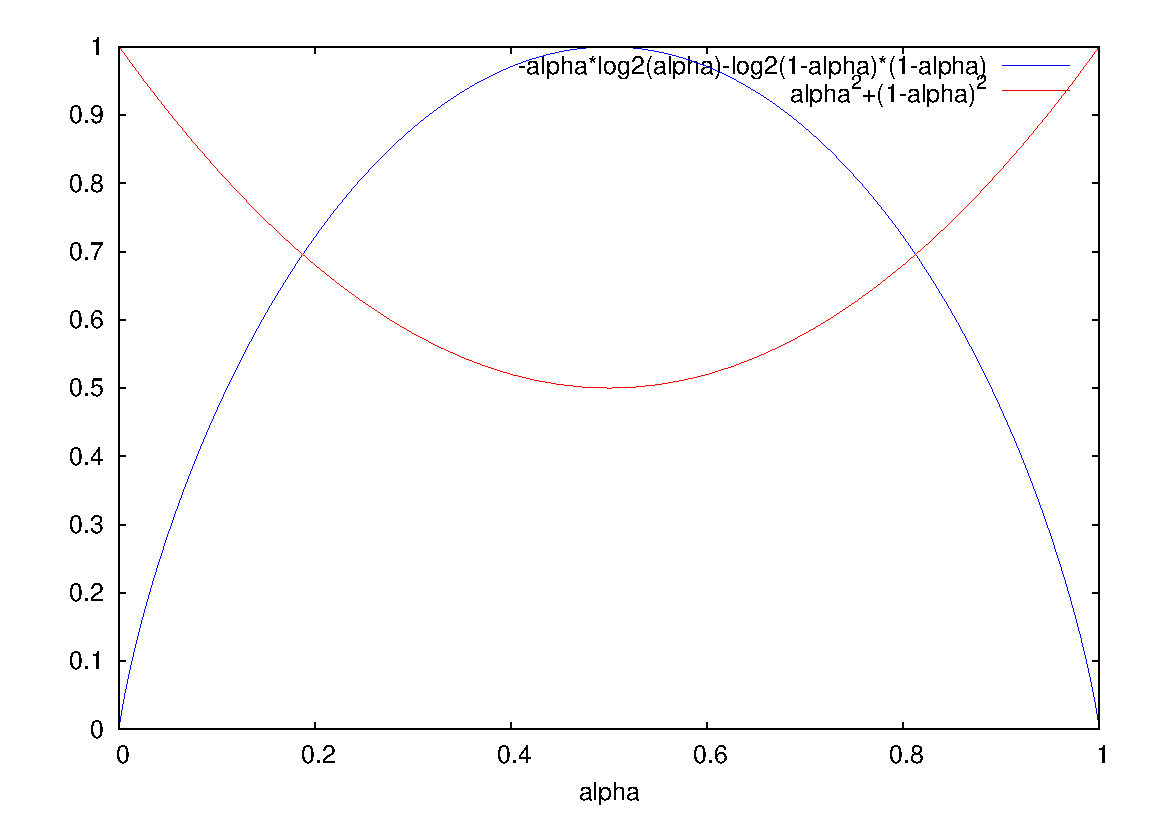
\includegraphics[width=.5\linewidth]{figs/entropy_purity}
\end{dmath}
\end{boxedminipage}%
\lthtmlfigureZ
\lthtmlcheckvsize\clearpage}

\stepcounter{section}
\stepcounter{subsection}
\stepcounter{subsubsection}
\stepcounter{subsubsection}
\stepcounter{subsubsection}
\stepcounter{subsection}
\stepcounter{subsubsection}
\stepcounter{subsubsection}
\stepcounter{section}
\stepcounter{subsection}
{\newpage\clearpage
\lthtmlfigureA{boxedminipage5406}%
\begin{boxedminipage}{2.0\linewidth}
\begin{verbatim}

(%i2) assume(alpha>0,1-alpha>0,beta>0,1-beta>0);
\end{verbatim}

\begin{dmath}[number={\%o2}]
 \left[ \alpha>0,\linebreak[0]\alpha<1,\linebreak[0]\beta>0,\linebreak[0]\beta<1 \right] \end{dmath}
\begin{verbatim}

(%i3) a : schmidt_ket(alpha);
\end{verbatim}

\begin{dmath}[number={\%o3}]
 \pmatrix{\sqrt{\alpha}\cr 0\cr 0\cr \sqrt{1-\alpha}\cr }\end{dmath}
\begin{verbatim}

(%i4) b : schmidt_ket(beta);
\end{verbatim}

\begin{dmath}[number={\%o4}]
 \pmatrix{\sqrt{\beta}\cr 0\cr 0\cr \sqrt{1-\beta}\cr }\end{dmath}
\end{boxedminipage}%
\lthtmlfigureZ
\lthtmlcheckvsize\clearpage}

{\newpage\clearpage
\lthtmlfigureA{boxedminipage5428}%
\begin{boxedminipage}{2.0\linewidth}
\begin{verbatim}

(%i5)  declare([u00,u01,u10,u11], complex);
\end{verbatim}

\begin{dmath}[number={\%o5}]
 \mathbf{done}\end{dmath}
\begin{verbatim}

(%i6) u : ket(u00,u01,u10,u11);
\end{verbatim}

\begin{dmath}[number={\%o6}]
 \pmatrix{\mathrm{u00}\cr \mathrm{u01}\cr \mathrm{u10}\cr \mathrm{u11}\cr }\end{dmath}
\end{boxedminipage}%
\lthtmlfigureZ
\lthtmlcheckvsize\clearpage}

{\newpage\clearpage
\lthtmlfigureA{boxedminipage5442}%
\begin{boxedminipage}{2.0\linewidth}
\begin{verbatim}

(%i7) rho : conjsimp((ident(2) otimes proj(u) otimes ident(2)) . proj(a otimes b))$,
\end{verbatim}

\end{boxedminipage}%
\lthtmlfigureZ
\lthtmlcheckvsize\clearpage}

{\newpage\clearpage
\lthtmlfigureA{boxedminipage5456}%
\begin{boxedminipage}{2.0\linewidth}
\begin{verbatim}

(%i8) rho_14 : ptrace(rho,2,3);
\end{verbatim}

\begin{dmath}[number={\%o8},style={\tiny }]
 \pmatrix{\alpha\*\beta\*\left| \mathrm{u00}\right| ^{2}&\linebreak[0]\alpha\*\sqrt{1-\beta}\*\sqrt{\beta}\*\mathrm{u00}^{\star}\*\mathrm{u01}&\linebreak[0]\sqrt{1-\alpha}\*\sqrt{\alpha}\*\beta\*\mathrm{u00}^{\star}\*\mathrm{u10}&\linebreak[0]\sqrt{1-\alpha}\*\sqrt{\alpha}\*\sqrt{1-\beta}\*\sqrt{\beta}\*\mathrm{u00}^{\star}\*\mathrm{u11}\cr \alpha\*\sqrt{1-\beta}\*\sqrt{\beta}\*\mathrm{u00}\*\mathrm{u01}^{\star}&\linebreak[0]\left(\alpha-\alpha\*\beta\right)\*\left| \mathrm{u01}\right| ^{2}&\linebreak[0]\sqrt{1-\alpha}\*\sqrt{\alpha}\*\sqrt{1-\beta}\*\sqrt{\beta}\*\mathrm{u01}^{\star}\*\mathrm{u10}&\linebreak[0]\left(\sqrt{1-\alpha}\*\sqrt{\alpha}-\sqrt{1-\alpha}\*\sqrt{\alpha}\*\beta\right)\*\mathrm{u01}^{\star}\*\mathrm{u11}\cr \sqrt{1-\alpha}\*\sqrt{\alpha}\*\beta\*\mathrm{u00}\*\mathrm{u10}^{\star}&\linebreak[0]\sqrt{1-\alpha}\*\sqrt{\alpha}\*\sqrt{1-\beta}\*\sqrt{\beta}\*\mathrm{u01}\*\mathrm{u10}^{\star}&\linebreak[0]\left(1-\alpha\right)\*\beta\*\left| \mathrm{u10}\right| ^{2}&\linebreak[0]\left(1-\alpha\right)\*\sqrt{1-\beta}\*\sqrt{\beta}\*\mathrm{u10}^{\star}\*\mathrm{u11}\cr \sqrt{1-\alpha}\*\sqrt{\alpha}\*\sqrt{1-\beta}\*\sqrt{\beta}\*\mathrm{u00}\*\mathrm{u11}^{\star}&\linebreak[0]\left(\sqrt{1-\alpha}\*\sqrt{\alpha}-\sqrt{1-\alpha}\*\sqrt{\alpha}\*\beta\right)\*\mathrm{u01}\*\mathrm{u11}^{\star}&\linebreak[0]\left(1-\alpha\right)\*\sqrt{1-\beta}\*\sqrt{\beta}\*\mathrm{u10}\*\mathrm{u11}^{\star}&\linebreak[0]\left(\left(\alpha-1\right)\*\beta-\alpha+1\right)\*\left| \mathrm{u11}\right| ^{2}\cr }\end{dmath}
\end{boxedminipage}%
\lthtmlfigureZ
\lthtmlcheckvsize\clearpage}

{\newpage\clearpage
\lthtmlfigureA{boxedminipage5499}%
\begin{boxedminipage}{2.0\linewidth}
\begin{verbatim}

(%i9) rho_4 : ptrace(rho,1,2,3);
\end{verbatim}

\begin{dmath}[number={\%o9}]
 \pmatrix{\left(1-\alpha\right)\*\beta\*\left| \mathrm{u10}\right| ^{2}+\alpha\*\beta\*\left| \mathrm{u00}\right| ^{2}&\linebreak[0]\left(1-\alpha\right)\*\sqrt{1-\beta}\*\sqrt{\beta}\*\mathrm{u10}^{\star}\*\mathrm{u11}+\alpha\*\sqrt{1-\beta}\*\sqrt{\beta}\*\mathrm{u00}^{\star}\*\mathrm{u01}\cr \left(1-\alpha\right)\*\sqrt{1-\beta}\*\sqrt{\beta}\*\mathrm{u10}\*\mathrm{u11}^{\star}+\alpha\*\sqrt{1-\beta}\*\sqrt{\beta}\*\mathrm{u00}\*\mathrm{u01}^{\star}&\linebreak[0]\left(\left(\alpha-1\right)\*\beta-\alpha+1\right)\*\left| \mathrm{u11}\right| ^{2}+\left(\alpha-\alpha\*\beta\right)\*\left| \mathrm{u01}\right| ^{2}\cr }\end{dmath}
\end{boxedminipage}%
\lthtmlfigureZ
\lthtmlcheckvsize\clearpage}

{\newpage\clearpage
\lthtmlfigureA{boxedminipage5515}%
\begin{boxedminipage}{2.0\linewidth}
\begin{verbatim}

(%i10) ket_to_mat(iket) := matrix([iket[1,1],iket[2,1]],[iket[3,1],iket[4,1]])$
\end{verbatim}

\end{boxedminipage}%
\lthtmlfigureZ
\lthtmlcheckvsize\clearpage}

{\newpage\clearpage
\lthtmlfigureA{boxedminipage5520}%
\begin{boxedminipage}{2.0\linewidth}
\begin{verbatim}

(%i11) mu : ket_to_mat(u)$
(%i12) X :  ket_to_mat(a) . mu . ket_to_mat(b);
\end{verbatim}

\begin{dmath}[number={\%o12}]
 \pmatrix{\sqrt{\alpha}\*\sqrt{\beta}\*\mathrm{u00}&\linebreak[0]\sqrt{\alpha}\*\sqrt{1-\beta}\*\mathrm{u01}\cr \sqrt{1-\alpha}\*\sqrt{\beta}\*\mathrm{u10}&\linebreak[0]\sqrt{1-\alpha}\*\sqrt{1-\beta}\*\mathrm{u11}\cr }\end{dmath}
\begin{verbatim}

(%i13) rho_4a : conjsimp( ctranspose(X) . X );
\end{verbatim}

\begin{dmath}[number={\%o13}]
 \pmatrix{\left(1-\alpha\right)\*\beta\*\left| \mathrm{u10}\right| ^{2}+\alpha\*\beta\*\left| \mathrm{u00}\right| ^{2}&\linebreak[0]\left(1-\alpha\right)\*\sqrt{1-\beta}\*\sqrt{\beta}\*\mathrm{u10}^{\star}\*\mathrm{u11}+\alpha\*\sqrt{1-\beta}\*\sqrt{\beta}\*\mathrm{u00}^{\star}\*\mathrm{u01}\cr \left(1-\alpha\right)\*\sqrt{1-\beta}\*\sqrt{\beta}\*\mathrm{u10}\*\mathrm{u11}^{\star}+\alpha\*\sqrt{1-\beta}\*\sqrt{\beta}\*\mathrm{u00}\*\mathrm{u01}^{\star}&\linebreak[0]\left(\left(\alpha-1\right)\*\beta-\alpha+1\right)\*\left| \mathrm{u11}\right| ^{2}+\left(\alpha-\alpha\*\beta\right)\*\left| \mathrm{u01}\right| ^{2}\cr }\end{dmath}
\end{boxedminipage}%
\lthtmlfigureZ
\lthtmlcheckvsize\clearpage}

{\newpage\clearpage
\lthtmlfigureA{boxedminipage5541}%
\begin{boxedminipage}{2.0\linewidth}
\begin{verbatim}

(%i14) is ( ratsimp(rho_4a) = ratsimp(rho_4) );
\end{verbatim}

\begin{dmath}[number={\%o14}]
 \mathbf{true}\end{dmath}
\end{boxedminipage}%
\lthtmlfigureZ
\lthtmlcheckvsize\clearpage}

{\newpage\clearpage
\lthtmlfigureA{boxedminipage5547}%
\begin{boxedminipage}{2.0\linewidth}
\begin{verbatim}

(%i15) P1 : conjsimp( mat_trace(rho));
\end{verbatim}

\begin{dmath}[number={\%o15}]
 \left(\left(\alpha-1\right)\*\beta-\alpha+1\right)\*\left| \mathrm{u11}\right| ^{2}+\left(1-\alpha\right)\*\beta\*\left| \mathrm{u10}\right| ^{2}+\left(\alpha-\alpha\*\beta\right)\*\left| \mathrm{u01}\right| ^{2}+\alpha\*\beta\*\left| \mathrm{u00}\right| ^{2}\end{dmath}
\end{boxedminipage}%
\lthtmlfigureZ
\lthtmlcheckvsize\clearpage}

{\newpage\clearpage
\lthtmlfigureA{boxedminipage5552}%
\begin{boxedminipage}{2.0\linewidth}
\begin{verbatim}

(%i16) av : [alpha,1-alpha]$
(%i17) bv : [beta,1-beta] $
(%i18) P2 : apply( "+", create_list( av[i] * abs(mu[i,j])^2 * bv[j], i,[1,2],j,[1,2]));
\end{verbatim}

\begin{dmath}[number={\%o18}]
 \left(1-\alpha\right)\*\left(1-\beta\right)\*\left| \mathrm{u11}\right| ^{2}+\left(1-\alpha\right)\*\beta\*\left| \mathrm{u10}\right| ^{2}+\alpha\*\left(1-\beta\right)\*\left| \mathrm{u01}\right| ^{2}+\alpha\*\beta\*\left| \mathrm{u00}\right| ^{2}\end{dmath}.
\end{boxedminipage}%
\lthtmlfigureZ
\lthtmlcheckvsize\clearpage}

{\newpage\clearpage
\lthtmlfigureA{boxedminipage5572}%
\begin{boxedminipage}{2.0\linewidth}
\begin{verbatim}

(%i19) is (ratsimp(P1) = ratsimp(P2));
\end{verbatim}

\begin{dmath}[number={\%o19}]
 \mathbf{true}\end{dmath}
\end{boxedminipage}%
\lthtmlfigureZ
\lthtmlcheckvsize\clearpage}


\end{document}
